%----------------------------------------------------------------------------
\chapter{Tervezés}
\label{chp:design}
%----------------------------------------------------------------------------
Ebben a fejezetben 



\section{A labor modelljének tervezése}
\label{design_model}

\Aref{fig:designmodelparts}-es ábra mutatja meg, hogy milyen 3 részere vághatjuk a terítéshez szükséges modellt.

\begin{figure}[ht]
	\centering
	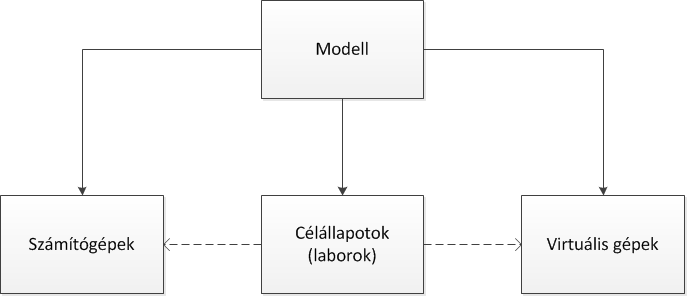
\includegraphics[width=100mm, keepaspectratio]{figures/design_modelparts.png}
	\caption{}
	\label{fig:designmodelparts}
\end{figure}

\Aref{fig:designcomputers}-s ábrán a számítógépeket tartalmazó darab részletesebb leírása van.

\begin{figure}[ht]
	\centering
	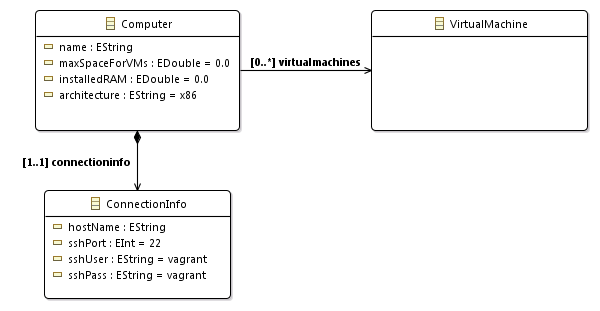
\includegraphics[width=110mm, keepaspectratio]{figures/design_computer.png}
	\caption{}
	\label{fig:designcomputers}
\end{figure}

\Aref{fig:designvm}-s ábrán a virtuális gépeket tartalmazó darab részletesebb leírása van.

\begin{figure}[ht]
	\centering
	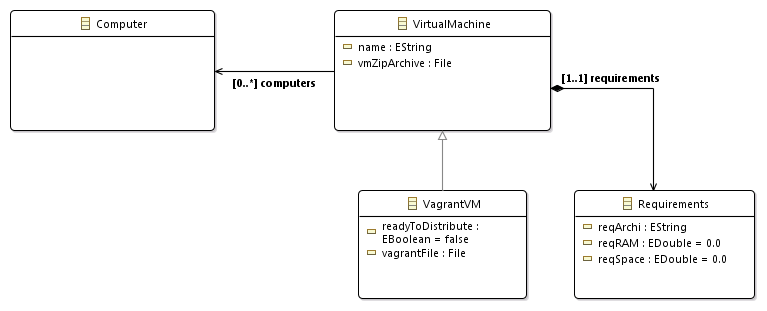
\includegraphics[width=130mm, keepaspectratio]{figures/design_vm.png}
	\caption{}
	\label{fig:designvm}
\end{figure}

\Aref{fig:designlab}-s ábrán a terítés végállapotát (pc->vm összerendelések) tartalmazó darab részletesebb leírása van.

\begin{figure}[h!]
	\centering
	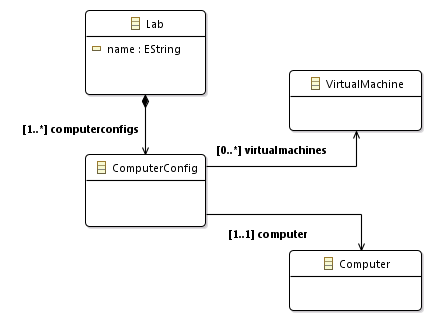
\includegraphics[width=100mm, keepaspectratio]{figures/design_lab.png}
	\caption{}
	\label{fig:designlab}
\end{figure}

\section{Terítési műveletek a modellen}

Annak a megtervezésére, hogy egy fájlterítési folyamat hogyan zajlik érdemes azt kisebb darabokba vágni, azt definiálni egyszerű műveletekkel.
Az előbbi fejezetben ismertetett modellre definiálok itt terítési műveleteket, és megkísérlem leírni segítségükkel az egész fájlterítési folyamatot.
Az egyszerű műveleteket a következő formátumban fogom definiálni: MŰVELET\_NEVE(paraméter1\_neve: paraméter1\_típusa, paraméter2\_neve\ldots).

A modellen értelmezett terítési műveletek: [a többi modellen értelmezhető művelet, amitől teljes rendszerré válik a dolog, de a terítésnél nem relevánsak kellenek-e? Gondolok itt azokra, amik üres modellt hoznak létre, hozzáadnak pc-t/vm-et/lab-et az erőforrásokhoz.]

\begin{itemize}
  \item KÜLÖNBSÉG(cél: Lab, erőforrások: LabSystem): Ez a művelet a paraméterei között különbséget képez, vagyis a Lab-ből kiszedi azokat a (Computer, VirtualMachine) párokat, amik a LabSystem-ben már szerepelnek. Ennek az a célja, hogy a terítendő VM-ek közül kiszűrje azokat, amelyek már ott vannak, ahova terítenénk őket. Visszatérési érték: Lab, ami a duplikátumokat nem tartalmazza.
  \item TÖRÖL(törlendő\_vm : VirtualMachine, melyik\_gépekről: List<Computer>): Ezzel a művelettel törölhetjük a második paraméter Computer-eket tartalmazó lista összes eleméről az adott virtuális gépet. Visszatérési érték: nincs, a paraméterként kapott gépeknek módosítja a tartalmát.
  \item KOMPATIBILIS\_E(pc: Computer, vm: VirtualMachine): Arra a kérdésre válaszol, hogy adot VM kompatibilis-e a Computer-rel. Ellenőrzi az architektúrák megfelelését, a memória és a szabad lemezterület méretét. Visszatérési érték: IGAZ vagy HAMIS.
  \item FELTÖLT(vm: VirtualMachine, pc: Computer): Feltölti a VM-et a Computer-re, vagyis hozzáadja annak a \code{virtualmachines} listájához. Visszatérési érték: nincs, amennyiben már ott található a feltöltendő VM a PC-n, akkor a művelet nem csinál semmit.
\end{itemize}

Az előbbiek segítségével már felírható a TERÍTÉS(cél: Lab, erőforrások: LabSystem) művelet: [talán ábrával és nem pszeudokóddal?]

\code{TERÍTÉS(cél: Lab, erőforrások: LabSystem):}\\
\indent \code{duplikátumok\_nélküli\_cél = KÜLÖNBSÉG(cél, LabSystem)}\\
\indent \indent \code{FOR minden ComputerConfig a duplikátumok\_nélküli\_cél-ban}\\
\indent \indent \indent	\code{FOR minden VirtualMachine a ComputerConfig.Virtualmachines-ben}\\
\indent \indent \indent	\code{HA(KOMPATIBILIS(ComputerConfig.Computer, VirtualMachine))}\\
\indent \indent \indent \indent	\code{AKKOR FELTÖLT(VirtualMachine, ComputerConfig.Computer)}


\section{Fájlterítő alkalmazás architektúrája}
\label{design_apparchi}

\Aref{fig:designoverview}-es ábra fogja elmagyarázni az új terítési megoldás alapvető működési elvét: beolvassuk a modellt, ami alapján az egyik gépet seed-nek kiválasztva megcsináljuk a torrentes terítés. Az alkalmazás a terítésben szereplő gépektől (a torrent swarm-ja) futás közben a terítés állapotáról kér le információkat.

\begin{figure}[ht]
	\centering
	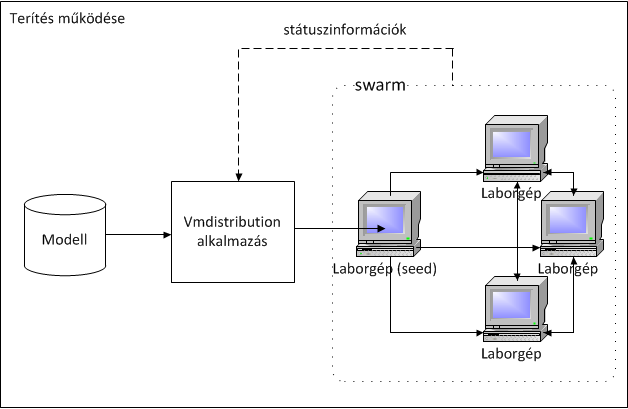
\includegraphics[width=130mm, keepaspectratio]{figures/design_overview.png}
	\caption{}
	\label{fig:designoverview}
\end{figure}

\Aref{fig:designprotocols}-es ábrán látjuk, hogy a terítés egyes szereplői hogyan és milyen protokollokat használva kommunikálnak egymással. [kell-e vajon ehhez, ill. az előzőhöz a tárhely, ahol a virtuális gépeket tároljuk?]

\begin{figure}[ht]
	\centering
	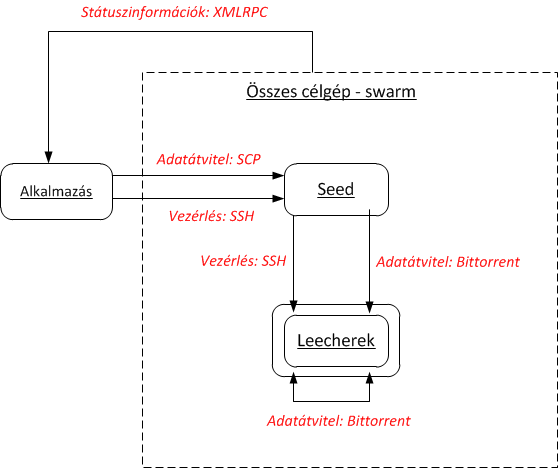
\includegraphics[width=140mm, keepaspectratio]{figures/design_protocols.png}
	\caption{.}
	\label{fig:designprotocols}
\end{figure}

